\documentclass[10pt]{article}
\usepackage[utf8]{inputenc}
\usepackage[T1]{fontenc}
\usepackage{amsmath}
\usepackage{amsfonts}
\usepackage{amssymb}
\usepackage[version=4]{mhchem}
\usepackage{stmaryrd}
\usepackage{graphicx}
\usepackage[export]{adjustbox}
\graphicspath{ {./images/} }
\usepackage{multirow}

\begin{document}
which takes two nonnegative integers as input, then the random variable $f(X, Y)$ has probability distribution function

$$
\operatorname{Pr}(f(X, Y)=z):=\sum_{\substack{x=0, y=0: \\ f(x, y)=z}}^{\infty} \operatorname{Pr}(X=x \text { and } Y=y)
$$

An example of such a function is addition. Define $Z:=X+Y$ where $X$ and $Y$ are independent, then the probability distribution $p_{Z}$ of $Z$ is given by the convolution of the distributions $p_{X}$ and $p_{Y}$, denoted as $p_{Z}=p_{X} * p_{Y}$, which means [52]

$$
p_{Z}(z)=\operatorname{Pr}(Z=z)=\sum_{x=0}^{z} p_{X}(x) \cdot p_{Y}(z-x)
$$

The convolution operator * is associative $((a * b) * c=a *(b * c))$ and thus writing $a * b * c$ is well-defined, for functions $a, b, c$ from the nonnegative integers to the real numbers. In general, the probability distribution of sums of independent random variables equals the convolutions of their individual probability distribution functions.

\section*{III. RECURSIVE EXPRESSIONS FOR THE WAITING TIME AND FIDELITY AS A RANDOM VARIABLE}
In this section, we derive expressions for the waiting time and fidelity of the first generated end-to-end link in the SWAP-ONLY repeater chain protocol. First, in sec. III-A, we derive a recursive definition for the random variable $T_{n}$, which represents the waiting time in a $2^{n}$-segment repeater chain. Section III-B is devoted to extending this definition to the Werner parameter $W_{n}$ of the pair, which stands in one-to-one correspondence to its fidelity $F_{n}$ using eq. (2):


\begin{equation*}
F_{n}=\left(1+3 W_{n}\right) / 4 \tag{7}
\end{equation*}


In sec. III-C, we show how to include the communication time after the entanglement swap and in sec. III-D, we extend the analysis of the waiting time and Werner parameter in the SWAP-ONLY protocol to the $d$-DIST-SWAP scheme.

\section*{A. Recursive expression for the waiting time in the SWAP-ONLY protocol}
In the following, we will derive a recursive expression for the waiting time $T_{n}$ of a SWAP-ONLY repeater chain of $2^{n}$ segments (see also fig. 1).

Before stating the expression, let us note that all three operations in the repeater chain protocols we study in this work, entanglement generation over a single hop, distillation and swapping, take a duration that is a multiple of $L_{0} / c$, the time to send information over a single segment (see sec. II-B for our assumptions on the duration of operations). For this reason, it is common to denote the waiting time in discrete units of $L_{0} / c$, which is a convention we comply with for $T_{n}$.

Let us first state the description of $T_{n}$ before explaining it.

\section*{Waiting time in the SWAP-ONLY protocol}
We recursively describe the random variable $T_{n}$ that represents the waiting time until the first endto-end link in a $2^{n}$-segment SWAP-ONLY repeater chain is generated, for $n \in\{0,1, \ldots\}$. The waiting time $T_{0}$ for generating point-to-point entanglement follows a geometric distribution with parameter $p_{\text {gen }}$. At the recursive step, the waiting time is given as the geometric compound sum


\begin{equation*}
T_{n+1}:=\sum_{j=1}^{K_{n}} M_{n}^{(j)} \tag{8}
\end{equation*}


where $M_{n}$ is an auxiliary random variable given by


\begin{equation*}
M_{n}:=g_{\mathrm{T}}\left(T_{n}^{(A)}, T_{n}^{(B)}\right) \tag{9}
\end{equation*}


and the function $g_{\mathrm{T}}$ is defined as


\begin{equation*}
g_{\mathrm{T}}\left(t_{A}, t_{B}\right):=\max \left\{t_{A}, t_{B}\right\} \tag{10}
\end{equation*}


The sum in eq. (8) is taken over the number of entanglement swaps $K_{n}$ until the first success, which is geometrically distributed with parameter $p_{\text {swap }}$ for every $n$. See fig. 1 for a depiction of $T_{n}$ and $K_{n}$.

Let us now elaborate on each of the steps in the expression of $T_{n}$.

We start with the base case $T_{0}$, the waiting time for the generation of elementary entanglement. Since we model the generation of single-hop entanglement by attempts which succeed with a fixed probability $p_{\text {gen }}$ (see sec. II-B), the waiting time $T_{0}$ is a discrete random variable (in units of $L_{0} / c$ ) which follows a geometric distribution with probability distribution given by $\operatorname{Pr}\left(T_{0}=t\right)=p_{\text {gen }}\left(1-p_{\text {gen }}\right)^{t-1}$ for $t \in\{1,2,3, \ldots\}$. For what follows, it will be more convenient to specify $T_{0}$ by its cumulative distribution function


\begin{equation*}
\operatorname{Pr}\left(T_{0} \leq t\right)=1-\left(1-p_{\text {gen }}\right)^{t} \tag{11}
\end{equation*}


Let us now assume that we have found an expression for $T_{n}$ and we want to construct $T_{n+1}$. In order to perform the entanglement swap to produce a single $2^{n+1}$-hop link, a node needs to wait for the production of two $2^{n}$-hop links, one on each side. Denote the waiting time for one of the pairs by $T_{n}^{(A)}$ and the other by $T_{n}^{(B)}$, both of which are i.i.d. with $T_{n}$. The time until both pairs are available is now given by $M_{n}:=\max \left(T_{n}^{(A)}, T_{n}^{(B)}\right)$ which is distributed according to


\begin{align*}
\operatorname{Pr}\left(M_{n} \leq t\right) & =\operatorname{Pr}\left(T_{n}^{(A)} \leq t \text { and } T_{n}^{(B)} \leq t\right) \\
& =\operatorname{Pr}\left(T_{n} \leq t\right)^{2} \tag{12}
\end{align*}


where the last equality follows from the fact that $T_{n}^{(A)}, T_{n}^{(B)}$ and $T_{n}$ are pairwise i.i.d. Since we assume that both the duration of the Bell-state measurement and the communication time of the heralding signal after the entanglement swap are negligible (see sec. II-B), $M_{n}$ is also the time at which the entanglement swap ends. We will drop the assumption on negligible communication time in sec. III-C.

In order to find the relation between $M_{n}$ and $T_{n+1}$, first note that the number of swaps $K_{n}$ at level $n$ until the first successful swap follows a geometric distribution with parameter $p_{\text {swap }}$. This is a direct consequence of our choice to model the success probability $p_{\text {swap }}$ to be independent of the state of the two input links (see sec. II-B). Next, recall that the two input links of a failing entanglement swap are lost and need to be regenerated. The regeneration of fresh entanglement after each failing entanglement swap adds to the waiting time. Thus, $T_{n+1}$ is a compound random variable: it is the sum of $K_{n}$ copies of $M_{n}$. Since the number of entanglement swaps $K_{n}$ is geometrically distributed, we say that $T_{n+1}$ is a geometric compound sum of $K_{n}$ copies of $M_{n}$. To be precise, we write


\begin{equation*}
T_{n+1}=\sum_{k=1}^{K_{n}} M_{n}^{(k)} \tag{13}
\end{equation*}


which means that the probability distribution of the waiting time $T_{n+1}$ is computed as the marginal of the waiting time conditioned on a fixed number of swaps:

$$
\operatorname{Pr}\left(T_{n+1}=t\right)=\sum_{k=1}^{\infty} \operatorname{Pr}\left(K_{n}=k\right) \cdot \operatorname{Pr}\left[\left(\sum_{j=1}^{k} M_{n}^{(j)}\right)=t\right]
$$

where the $M_{n}^{(j)}$ are copies of $M_{n}$.

The waiting time $T_{n}$ is the same quantity as was studied by Shchukin et al. [45]. Indeed, in sec. VI, we show that our algorithms for computing the probability distribution of $T_{n}$ recover their numerical results.

\section*{B. Joint recursive expression of waiting time and Werner parameter for the SWAP-ONLY protocol}
In this section, we extend the expression of the waiting time for the first end-to-end link produced using the SWAP-ONLY protocol with the link's state. To be precise, we give a recursive expression for the waiting time $T_{n}$ and Werner parameter $W_{n}$ of this state, which is well-defined since all states that the SWAP-ONLY repeater chain protocol holds at any time during its execution are Werner states. The latter statement is a direct consequence of the fact that in our modeling, all operations in the SWAP-ONLY protocol only output Werner states: we choose to model the generated single-hop entanglement as Werner states and furthermore the class of Werner states is invariant under memory errors and entanglement swaps (see sec. II-B). The fidelity $F_{n}$ of the first end-to-end state on $2^{n}$ segments can be computed from its Werner parameter using eq. (7).

We express the waiting time and Werner parameter as a joint random variable $\left(T_{n}, W_{n}\right)$. Describing the two as a tuple allows us to capture the fact that the Werner parameter of a link depends on the time it was produced at. In sec. III-A, we found that the failure of multiple swapping attempts corresponds to the sum of their waiting times. In order to extend this description to the tuple of waiting time and Werner parameter, we define the forgetting sum $\widehat{\sum}$ on sequences of tuples $\left\{\left(x_{j}, y_{j}\right) \mid 1 \leq j \leq m\right\}$ for some $m \in\{1,2, \ldots\}$ as


\begin{equation*}
\widehat{\sum}_{j=1}^{m}\left(x_{j}, y_{j}\right):=\left(\sum_{j=1}^{m} x_{j}, y_{m}\right) \tag{14}
\end{equation*}


In analogy to the geometric compound sum from eq. (13), we define the geometric compound forgetting sum $\left(X^{\prime}, Y^{\prime}\right):=\widehat{\sum}_{j=1}^{K}(X, Y)$, which formally means

$$
\begin{aligned}
& \operatorname{Pr}\left(X^{\prime}=x \text { and } Y^{\prime}=y\right) \\
& =\sum_{k=1}^{\infty} p(1-p)^{k-1} \cdot \operatorname{Pr}\left(\widehat{\sum}_{j=1}^{k}(X, Y)^{(j)}=(x, y)\right)
\end{aligned}
$$

where $X$ and $Y$ and their primed version are random variables, and $K$ is a geometrically distributed random variable with parameter $p$.

Making use of the compound forgetting sum, we give the expression for the joint random variable of waiting time $T_{n}$ and Werner parameter $W_{n}$.

\section*{Waiting time and Werner parameter in the SWAP-ONLY protocol}
The joint random variable $\left(T_{n}, W_{n}\right)$ is defined as follows. The waiting time $T_{0}$ is the same as in sec. III-A and $\operatorname{Pr}\left(W_{0}=w_{0}\right)=1$ where $w_{0} \in[0,1]$ is some pre-specified constant that determines the state of the single-hop entanglement that is produced between adjacent nodes. At the recursive step, the waiting time and Werner parameter are given by the geometric compound forgetting sum

\begin{center}
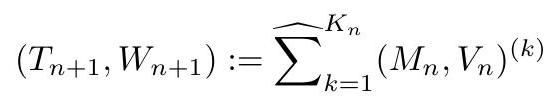
\includegraphics[max width=\textwidth]{2024_06_11_851f269fc4a3fe65b610g-2}
\end{center}

where, as in sec. III-A, $K_{n}$ follows a geometric distribution with parameter $p_{\text {swap }}$. The auxiliary joint random variable $\left(M_{n}, V_{n}\right)$ is defined as


\begin{equation*}
\left(M_{n}, V_{n}\right):=g\left(\left(T_{n}, W_{n}\right)^{(A)},\left(T_{n}, W_{n}\right)^{(B)}\right) \tag{16}
\end{equation*}


The function $g$ is given by


\begin{align*}
& g\left(\left(t_{A}, w_{A}\right),\left(t_{B}, w_{B}\right)\right):=  \tag{17}\\
& \quad\left(g_{\mathrm{T}}\left(t_{A}, t_{B}\right), g_{\mathrm{W}}\left(\left(t_{A}, w_{A}\right),\left(t_{B}, w_{B}\right)\right)\right)
\end{align*}


where $g_{\mathrm{T}}$ is defined in eq. 10 and

$g_{\mathrm{W}}\left(\left(t_{A}, w_{A}\right),\left(t_{B}, w_{B}\right)\right):=w_{A} \cdot w_{B} \cdot e^{-\left|t_{A}-t_{B}\right| / T_{\text {coh }}}$

with $T_{\text {coh }}$ the quantum memory coherence time as described in sec. II-B.

We now explain the above expressions. For a single segment ( $n=0$ ), the waiting time and Werner parameter are uncorrelated because we model the attempts at generating singlehop entanglement to be independent and to each take equally long (see sec. II-B). At the recursive step, an entanglement swap which produces $2^{n+1}$-hop entanglement requires the generation of two $2^{n}$-hop links. The expression for the waiting time $T_{n+1}$ is identical to eq. (8) in sec. III-A. In order to argue that eq. (15) also gives the correct expression for $W_{n+1}$, we first show that the Werner parameter of the output link of an entanglement swap is given by $V_{n}$ in eq. (16), provided the swap succeeded. Since $M_{n}$ as defined in eq. (16) is identical to its expression in eq. (9) in sec. III-A, we only need to argue\\
why $g_{\mathrm{W}}$ in eq. (18) correctly computes the Werner parameter of the output link after an entanglement swap.

In order to do so, denote by $A$ and $B$ the input links to the entanglement swap and denote by $\left(t_{A}, w_{A}\right)$ and $\left(t_{B}, w_{B}\right)$ their respective delivery times and Werner parameters. Without loss of generality, choose $t_{A} \geq t_{B}$, i.e. link $A$ is produced after link $B$. Link $A$ is produced last, so the entanglement swap will be performed directly after its generation and hence link $A$ will enter the entanglement swap with Werner parameter $w_{A}$. Link $B$ is produced earliest and will therefore decohere until production of link $A$. It follows from eq. (3) that $B$ 's Werner parameter immediately before the swap equals


\begin{equation*}
w_{B}^{\prime}=w_{B} \cdot e^{-\left|t_{A}-t_{B}\right| / T_{\mathrm{coh}}} \tag{19}
\end{equation*}


Once two links have been delivered, the entanglement swap would produce the $2^{n+1}$-hop state with Werner parameter


\begin{equation*}
w_{A} \cdot w_{B}^{\prime} \tag{20}
\end{equation*}


as in eq. (4), provided the swap is successful. Combining eqs. (19) and (20) yields the definition of $g_{\mathrm{W}}$ in eq. (18).

Note that in the definition of $g_{\mathrm{W}}$ in eq. (18) we used the same assumption on the duration of the entanglement swap as in sec. III-A, i.e. that both the Bell-state measurement and the subsequent communication time are negligible (see also sec. II-B). This implies that $V_{n}$ in eq. (16) expresses the Werner parameter of the produced $2^{n+1}$-hop link in case the swap is successful. We treat the case of nonzero communication time in sec. III-C.

The last step in finding the Werner parameter $W_{n+1}$ in eq. (15) is to bridge the gap with ( $M_{n}, V_{n}$ ) from eq. (16). If the entanglement swap fails, then the $2^{n+1}$-hop link with its Werner parameter in eq. (20) will never be produced since both initial $2^{n}$-hop entangled pairs are lost. Instead, two fresh $2^{n}$-hop links will be generated. In order to find how the Werner parameter on level $n+1$ is expressed as a function of the waiting times and Werner parameters at level $n$, consider a sequence $\left(m_{j}, v_{j}\right)$ of waiting times $m_{j}$ and Werner parameters $v_{j}$, where $j$ runs from 1 to the first successful swap $k$. The $m_{j}$ correspond to the waiting time until the end of the entanglement swap that transforms two $2^{n}$-hop links into a single $2^{n+1}$-hop link and the $v_{j}$ to the output link's Werner parameter if the swap were successful. We have found in sec. III-A that the total waiting time is given by $\sum_{j=1}^{k} m_{j}$, the sum of the duration of the production of the lost pairs (see eq. (8)). Note, however, that the Werner parameter of the $2^{n+1}$ hop link is only influenced by the links that the successful entanglement swap acted upon. Since the entanglement swaps are performed until the first successful one, the output link is the last produced link and therefore its Werner parameter equals $v_{k}$. We thus find that the waiting time $t_{\text {final }}$ of the first $2^{n+1}$-hop link and its Werner parameter $w_{\text {final }}$ are given by the forgetting sum from eq. (14):

$$
\left(t_{\text {final }}, w_{\text {final }}\right)=\left(\sum_{j=1}^{k} m_{j}, v_{k}\right)={\widehat{\sum_{j=1}}}_{j}^{k}\left(m_{j}, v_{j}\right)
$$

Taking into account that the number of swaps $k$ that need to be performed until the first successful one is an instance of the random variable $K_{n}$, we arrive at the full recursive expression for the waiting time and Werner parameter at level $n+1$ as given in eq. (15).

It is not hard to see that the projection $\left(T_{n}, W_{n}\right) \mapsto T_{n}$ recovers the definition of waiting time from III-A. Indeed, following the recursive definition of $\left(T_{n}, W_{n}\right)$ in eqs. (15)(18), the waiting time $T_{n}$ is not affected by the Werner parameters $W_{\ell}$ at lower nesting levels $\ell<n$.

\section*{C. Including communication time}
While deriving the expressions for waiting time and Werner parameter of the first produced end-to-end link in secs. III-A and III-B, we have explicitly assumed that the total time the entanglement swap takes is negligible. Here, we include the communication time of the heralding signal from the entanglement swap into the expressions for $M_{n}$ and $V_{n}$ (eqs. (9) and (16)), which represent the waiting time and Werner parameter directly after the entanglement swap if it were successful. This communication time equals $2^{n}$ time steps (in units of $L_{0} / c$ ) for a swap that transforms two $2^{n}$-hop links into a single $2^{n+1}$ hop link (see sec. II-B). The expressions for $M_{n}$ and $V_{n}$ are modified by replacing $g_{\mathrm{T}}$ in eq. 10 by


\begin{equation*}
g_{\mathrm{T}}^{n}\left(t_{A}, t_{B}\right):=g_{\mathrm{T}}\left(t_{A}, t_{B}\right)+2^{n} \tag{21}
\end{equation*}


and replacing $g_{\mathrm{W}}$ from eq. (18) by


\begin{align*}
& g_{\mathrm{W}}^{n}\left(\left(t_{A}, w_{A}\right),\left(t_{B}, w_{B}\right)\right) \\
& \quad:=g_{\mathrm{W}}\left(\left(t_{A}, w_{A}\right),\left(t_{B}, w_{B}\right)\right) \cdot e^{-2^{n} / T_{\mathrm{coh}}} \tag{22}
\end{align*}


Equation (21) expresses that the entanglement swap takes $2^{n}$ timesteps longer, while eq. (22) captures the decoherence of the state during the communication time of the entanglement swap, following eq. (3).

\section*{D. Waiting time and Werner parameter for the $d$-DIST-SWAP protocol}
In this section, we sketch how to extend the expression of the waiting time $T_{n}$ and Werner parameter $W_{n}$ from secs. III-A-III-C to the case of the $d$-DIST-SWAP repeater protocol presented in sec. II-A. Recall that the $d$-DIST-SWAP protocol is identical to the SWAP-ONLY protocol except for the fact that each entanglement swap is performed on the output of a recurrence distillation scheme with $d$ nesting levels. By a $d^{\prime}$-distilled $2^{n}$-hop link we denote a $2^{n}$-hop link which is the result of successful entanglement distillation on two $\left(d^{\prime}-1\right)$ distilled $2^{n}$-hop links and by a 0 -distilled $2^{n}$-hop link we mean a link that is the result of a successful entanglement swap on two $2^{n}$-hop links. Thus, every entanglement swap in the $d$-DIST-SWAP protocol is performed on $d$-distilled links only.

Note that at every level of the nested swapping, there are $d$ levels of nested distillation. To tackle the 'double nesting' we modify the waiting time in the SWAP-ONLY protocol by splitting up the tuple of random variables $\left(T_{n}, W_{n}\right)$ in eq. (15), which represents the waiting time and Werner parameter at level $n$, into $d+1$ tuples of random variables $\left(T_{n}^{d^{\prime}}, W_{n}^{d^{\prime}}\right)$ for $d^{\prime} \in\{0,1, \ldots, d\}$. The random variable $T_{n}^{d^{\prime}}$ corresponds to the waiting time until the end of the first successful distillation\\
attempt on two $d^{\prime}$-distilled $2^{n}$-hop links, and $W_{n}^{d^{\prime}}$ to the link's Werner parameter.

We first analyze the recurrence distillation protocol at a single swapping nesting level and subsequently tie this analysis in with the nested swapping structure.

If we fix the nesting level $n$, we can straightforwardly apply the analysis of sec. III-B to the nested distillation. First, we define $\left(M_{n}^{d^{\prime}}, V_{n}^{d^{\prime}}\right)$, which characterizes a link after a single distillation attempt on two $2^{n}$-hop $d^{\prime}$-distilled links in case the attempt is successful. This joint random variable is the analogue of $\left(M_{n}, V_{n}\right)$ from eq. (16), which has the same interpretation but in this case for a swapping attempt. The analysis resulting in eq. (16) carries over and yields


\begin{equation*}
\left(M_{n}^{d^{\prime}}, V_{n}^{d^{\prime}}\right):=g_{\mathrm{D}}\left(\left(T_{n}^{d^{\prime}}, W_{n}^{d^{\prime}}\right)^{(A)},\left(T_{n}^{d^{\prime}}, W_{n}^{d^{\prime}}\right)^{(B)}\right) \tag{23}
\end{equation*}


where $g_{\mathrm{D}}$ is the analogue of $g$ in eq. (17) and describes how two input links are transformed into one high-quality link by a successful distillation step:

$$
g_{\mathrm{D}}\left(\left(t_{A}, w_{A}\right),\left(t_{B}, w_{B}\right)\right)=\left(g_{\mathrm{T}}\left(t_{A}, w_{A}\right), w\right)
$$

where

$$
w:= \begin{cases}w_{\text {dist }}\left(w_{A} \cdot e^{-\left|t_{A}-t_{B}\right| / T_{\text {coh }}}, w_{B}\right) & \text { if } t_{A} \leq t_{B} \\ w_{\text {dist }}\left(w_{A}, w_{B} \cdot e^{-\left|t_{A}-t_{B}\right| / T_{\text {coh }}}\right) & \text { if } t_{A}>t_{B}\end{cases}
$$

and $w_{\text {dist }}$ is given in eq. (5). The function $g_{\mathrm{D}}$ outputs a tuple of waiting time and Werner parameter of the output state after distillation. The waiting time requires two links to be generated and is thus given by $g_{\mathrm{T}}$ in eq. (10). The Werner parameter equals the Werner parameter of distillation as given by $w_{\text {dist }}$ in eq. (5) on the two input links, of which the earlier suffered decoherence as given in eq. (3).

The random variables $\left(T_{n}^{d^{\prime}}, W_{n}^{d^{\prime}}\right)$ correspond to the waiting time and Werner parameter after the first successful distillation attempt on two $d^{\prime}$-distilled $2^{n}$-hop links, so in line with the analysis leading to eq. (15) we obtain


\begin{equation*}
\left(T_{n}^{d^{\prime}+1}, W_{n}^{d^{\prime}+1}\right)={\widehat{\sum_{j=1}^{D^{d^{\prime}}}}}_{n}^{j}\left(M_{n}^{d^{\prime}}, V_{n}^{d^{\prime}}\right)^{(j)} \tag{24}
\end{equation*}


The random variable $\mathcal{D}_{n}^{d^{\prime}}$ corresponds to the number of distillation attempts with two $d^{\prime}$-distilled $2^{n}$-hop links as input, up to and including the first successful attempt. It is the analogue of $K_{n}$ in eq. (15), the number of swap attempts until the first success.

At this point, we have an expression for $\left(T_{n}^{d}, W_{n}^{d}\right)$, the waiting time and Werner parameter of the resulting link after performing a $d$-level recurrence protocol on 0 -distilled input links that each span $2^{n}$ hops. Since the recurrence protocol is performed at every swapping nesting level of the $d$-DIST-SWAP protocol, we can insert this expression into our previous analysis using the following two remarks. First, a 0 -distilled link is the output of an entanglement swap, so $\left(T_{n}^{0}, W_{n}^{0}\right)$ in the $d$-DIST-SWAP scheme takes the role that $\left(T_{n}, W_{n}\right)$ has in the SWAP-ONLY protocol:


\begin{equation*}
\left(T_{n}^{0}, W_{n}^{0}\right)=\left(T_{n}, W_{n}\right) \tag{25}
\end{equation*}


Second, since an entanglement swap takes as input two $d$ distilled links, we find that we should replace the definition of $\left(M_{n}, V_{n}\right.$ ) in eq. (16) by


\begin{equation*}
\left(M_{n}, V_{n}\right)=g\left(\left(T_{n}^{d}, W_{n}^{d}\right)^{(A)},\left(T_{n}^{d}, W_{n}^{d}\right)^{(B)}\right) \tag{26}
\end{equation*}


where $g$ is defined in eq. (17).

We finish this section by remarking that for the $d$-DIST-SWAP protocol, we cannot treat waiting time independently of the Werner parameter of the produced link, as we did for the SWAP-ONLY scheme in sec. III-A. The reason behind this is the following difference between the nested swaps and the nested distillation: in the former, the success probability $p_{\text {swap }}$ and therefore the number of swaps $K_{n}$ is independent of the time and state of the produced links, whereas the success probability of entanglement distillation is a function of their states (see eq. (6)). Consequently, the summation bound $\mathcal{D}_{n}^{d^{\prime}}$ and the Werner parameter $V_{n}^{d^{\prime}}$ in the summands $\left(M_{n}^{d^{\prime}}, V_{n}^{d^{\prime}}\right)$ in eq. (24) are correlated. Therefore, both the waiting time and Werner parameter at any swapping level depend on both waiting time and Werner parameter at the levels below.

\section*{IV. ALGORITHMS FOR COMPUTING WAITING TIME AND FIDELITY OF THE FIRST END-TO-END LINK}
In this section, we present two algorithms for determining the probability distribution of the waiting time $T_{n}$ and average Werner parameter $W_{n}$ of the first end-to-end link produced by the repeater chain (see sec. III). The first algorithm is a Monte Carlo algorithm which applies to both families of repeater chain protocols considered in this work: SWAP-ONLY and $d$-DIST-SWAP. The second algorithm only applies to the SWAP-ONLY protocol and is faster than the first. We summarize the runtime of the different algorithms presented in this section in table $\mathrm{I}$.

\section*{A. First algorithm: Monte Carlo simulation}
The first algorithm is a randomized function which produces a sample from the probability distribution of the joint random variable $\left(T_{n}, W_{n}\right)$. By running the algorithm many times, sufficient statistics can be produced to reconstruct the distribution of the joint random variable up to arbitrary precision (see below for a rigorous statement). We first outline the algorithm that samples from the waiting time in the SWAP-ONLY protocol following sec. III-A, after which we show how to extend it to track the Werner parameter (sec. III-B), how to include the communication time after a swap (sec. III-C) and how to adjust it for the $d$-DIST-SWAP protocol (sec. III-D). Pseudocode can be found in algorithm 1.

We start by explaining the Monte Carlo algorithm for the waiting time in the SWAP-ONLY protocol. Let $s(X)$ denote a randomized function that yields a sample from the random variable $X$. We remark that if the cumulative distribution function of $X$ is known, then sampling from $X$ can be done efficiently using inverse transform sampling, which is a standard technique to produce a sample from an arbitrary distribution by evaluating its inverse cumulative distribution function on a sample from the uniform distribution on the interval $[0,1]$.

\begin{center}
\begin{tabular}{|c|c|c|c|c|}
\hline
\multirow{2}{*}{}\begin{tabular}{l}
Repeater chain protocol \\
(sec. II-A) \\
\end{tabular} &  & \multirow{2}{*}{}\begin{tabular}{l}
Markov-chain-approach \\
[45]
[46] \\
[45]
\end{tabular} & \multicolumn{2}{|c|}{Algorithms in this work} \\
\hline
 &  &  & Monte-Carlo & Deterministic \\
\hline
\multirow{3}{*}{SWAP-ONLY} & \begin{tabular}{l}
Waiting time up to $99 \%$ of \\
the cumulative probabilities \\
\end{tabular} & $\Theta(\exp (N))$ & $\mathcal{O}(\operatorname{poly}(N))$ & $\Theta(\operatorname{poly}(N))$ \\
\hline
 & \begin{tabular}{l}
Waiting time up to \\
fixed truncation time $t_{\text {trunc }}=1000$ \\
\end{tabular} & $\Theta(\exp (N))$ & $\mathcal{O}(\operatorname{poly}(N))$ & $\Theta(\log (N))$ \\
\hline
 & Fidelity & $x$ & $\mathcal{O}(\operatorname{poly}(N))$ & $\Theta(\operatorname{poly}(N))$ \\
\hline
$d$-DIST-SWAP & Waiting time $\&$ fidelity & $x$ & $\mathcal{O}(\operatorname{poly}(N))$ & $x$ \\
\hline
\end{tabular}
\end{center}

TABLE I: The time complexity of the algorithms for computing waiting time and fidelity of entanglement distribution through repeater chains as presented in this work compared to existing algorithms. The algorithms have exponential (exp) or polynomial (poly) runtime in $N=2^{n}$, the number of segments in the repeater chain, for $n \in\{1,2, \ldots\}$. The Monte Carlo algorithm is a randomized algorithm; its presented runtime is the average runtime. The cross $(\times)$ indicates that the algorithm is not present.

We can thus construct the sampler from the waiting time for elementary entanglement, $T_{0}$, using the inverse of the cumulative distribution function of $T_{0}$ as given in eq. (11):


\begin{equation*}
s\left(T_{0}\right)=\left\lceil\log _{(1-p)}(1-s(U))\right\rceil \tag{27}
\end{equation*}


where $U$ is a random variable which is distributed uniformly at random on $[0,1]$ and $\lceil$.$\rceil denotes the ceiling function.$

For sampling from higher levels, we first note that we can easily transform a sampler $s(X)$ into a sampler $s_{\text {sum }}(X, p)$ from a geometric sum $\sum_{j=1}^{K} X^{(j)}$, where $K$ is geometrically distributed with parameter $p$. The sampler from the geometric sum probabilistically calls itself:

$$
s_{\text {sum }}(X, p):= \begin{cases}s(X) & \text { with prob. } p \\ s(X)+s_{\text {sum }}(X, p) & \text { with prob. } 1-p\end{cases}
$$

From the recursive expression for the waiting time $T_{n}$ in sec. III-A it now follows directly that we can construct a sampler from $T_{n}$ for $n \geq 1$ :

$$
s\left(T_{n}\right)=s_{\text {sum }}\left(M_{n}, p_{\text {swap }}\right)
$$

which, per definition of $s_{\text {sum }}$, makes a call to $s\left(M_{n}\right)$ which is given by

$$
s\left(M_{n}\right)=g_{\mathrm{T}}\left(s\left(T_{n-1}\right), s\left(T_{n-1}\right)\right)
$$

where $g_{\mathrm{T}}$ is defined in eq. (10).

Using the Dvoretzky-Kiefer-Wolfowitz inequality [53], we determine how many samples from $\left(T_{n}, W_{n}\right)$ we need in order to obtain bounds on its cumulative probabilities. It follows from this inequality that if $q(t):=\operatorname{Pr}\left(T_{n} \leq t\right)$ denotes the cumulative probability function of the waiting time $T_{n}$ and $q_{m}(t)$ the empirical cumulative probabilities after having drawn $m$ samples, then the difference between $q$ and $q_{m}$ is bounded as

$$
\operatorname{Pr}\left(\left|q(t)-q_{m}(t)\right|>\epsilon\right) \leq 2 e^{-2 m \epsilon^{2}}
$$

for all $t \geq 0$. Thus we can bound the probability that the empirical estimate $q_{m}(t)$ deviates from $q(t)$ at most $\epsilon$ for any value of $t$ by $z=2 e^{-2 m \epsilon^{2}}$ if the number of samples to draw equals


\begin{equation*}
m=-\log (z / 2) /\left(2 \epsilon^{2}\right) \tag{28}
\end{equation*}


Let us emphasize that this number of samples is independent of any parameters of the repeater chain, for instance the number of segments, and thus its contribution to the runtime or space usage of the Monte Carlo algorithm is at most a multiplicative constant, independent of any such parameters.

Following sec. III-B, we modify the Monte Carlo algorithm to also compute the Werner parameter of the sampled produced entangled pair (for pseudocode see algorithm 1). First note that the notation $s(X)$ which samples from a random variable $X$ can also be applied to a joint random variable $(X, Y)$, so that $s((X, Y))$ returns a tuple. We will now define a sampler $s\left(\left(T_{n}, W_{n}\right)\right)$ where $\left(T_{n}, W_{n}\right)$ is the joint random variable representing waiting time and Werner parameter of a $2^{n}$ segment SWAP-ONLY repeater chain (see sec. III-B). For this, we first need to adapt the sampler of the geometric compound sum $s_{\text {sum }}$ to a sampler of the geometric compound forgetting sum (eq. (14)) by defining $\hat{s}_{\text {sum }}((X, Y), p)$ where $X$ and $Y$ are arbitrary random variables and $p \in[0,1]$ is the parameter of the geometric distribution:

$$
\hat{s}_{\text {sum }}((X, Y), p):= \begin{cases}s((X, Y)) & \text { with prob. } p \\ \pi(s((X, Y)))+\hat{s}_{\text {sum }}((X, Y), p) \\ & \text { with prob. } 1-p\end{cases}
$$

where ' + ' denotes pairwise addition and $\pi$ is the projector onto the first element of a tuple: $\pi((x, y))=(x, 0)$ for any numbers $x, y$.

A recursive definition of the joint sampling function from $\left(T_{n}, W_{n}\right)$ follows directly from the joint expression for waiting time $T_{n}$ and Werner parameter $W_{n}$ in eqs. (15)-(18):

$$
\begin{aligned}
s\left(\left(T_{0}, W_{0}\right)\right) & =\left(s\left(T_{0}\right), w_{0}\right) \\
s\left(\left(T_{n}, W_{n}\right)\right) & =\hat{s}_{\text {sum }}\left(\left(M_{n}, V_{n}\right), p_{\text {swap }}\right) \\
s\left(\left(M_{n}, V_{n}\right)\right) & =g\left(s\left(T_{n-1}, W_{n-1}\right), s\left(T_{n-1}, W_{n-1}\right)(29)\right.
\end{aligned}
$$

where $w_{0}$ is the Werner parameter of each single-hop link at the time it is produced (see sec. II-B) and the function $g$ is defined in eq. (17). In this pseudocode for this Monte Carlo algorithm in algorithm 1 , the sampler $s\left(T_{n}, W_{n}\right)$ is denoted by sample\_swap.

Since the expression for $\left(T_{n}, W_{n}\right)$ from sec. III-B assumes that the communication time for the heralding signal after the entanglement swap takes negligible time, it is not included in the Monte Carlo algorithm above. Fortunately, the adaptation to include this communication time as in sec. III-C directly


\end{document}